\documentclass[11pt]{article}

\usepackage{amsmath,amssymb,amsfonts}
\usepackage{graphicx}
\usepackage{pgfplots}
\usepackage{multicol}
\usepackage{enumitem}
\usepgfplotslibrary{fillbetween}
\pgfplotsset{compat=1.16,width=10cm}


\setlength{\topmargin}{-.5in} \setlength{\textheight}{9.25in}
\setlength{\oddsidemargin}{0in} \setlength{\textwidth}{6.8in}


\begin{document}

\Large

\noindent{\bf Name: \hfill Date: \hfill Quiz 7 \hfill Precalculus - Hargus}

\medskip\hrule
\vspace{10pt}

\noindent \textbf{Instructions:} Please \textbf{show all work} (partial credit will be given for correct work, even if your answer is wrong).

\vspace{10pt}



\begin{enumerate}

\item (20 points) Use the graph of $f(x)$ below to answer the following questions.
\begin{center}
\begin{tikzpicture}[]
\begin{axis}[
  xlabel={$x$}, ylabel={$y$}
  ,axis lines=middle
  ,samples=1000, grid, thick,
  ymin=-1, ymax=4, ytick={-5,...,5}, ylabel=$y$,
  xmin=-1, xmax=5, xtick={-5,...,5}, xlabel=$x$,
  height=10cm, width=15cm,
]
\addplot[blue, domain=-1:2]{1/4 * \x^3 + 1};
\addplot[blue, domain=2:4]{-\x + 4};
\addplot[blue, domain=4:5]{\x - 4};

\end{axis}
\end{tikzpicture} 
\end{center}

\begin{enumerate}[itemsep=40pt, label={\alph*)}]
    \item Does $f'(0)$ (the derivative of $f(x)$ when $x=0$) exist? If yes, what does it equal?
    \item Does $f'(2)$ exist? If yes, what does it equal?
    \item Does $f'(3)$ exist? If yes, what does it equal?
    \item Does $f'(4)$ exist? If yes, what does it equal?
\end{enumerate}

\newpage

\item (15 points) Use the graph of $f(x)$ below to answer the following questions.
\begin{center}
\begin{tikzpicture}[]
\begin{axis}[
  xlabel={$x$}, ylabel={$y$}
  ,axis lines=middle
  ,samples=1000, grid, thick,
  ymin=-1, ymax=3, ytick={-5,...,5}, ylabel=$y$,
  xmin=-1, xmax=5.5, xtick={-5,...,5}, xlabel=$x$,
  height=9cm, width=14cm,
]
\addplot[blue, domain=0:2]{sqrt(-(x-2)^2 + 4)};
\addplot[blue, domain=2:4]{-\x + 4};
\addplot[blue, domain=4:5.5]{\x - 4};

\end{axis}
\end{tikzpicture} 
\end{center}

\begin{enumerate}[itemsep=0pt, label={\alph*)}]
    \item Find $\displaystyle \int_{2}^{5} f(x)dx$.
\vspace{50pt}
\begin{flushright}
$\displaystyle \int_{2}^{5} f(x)dx = \rule{2cm}{0.4pt}$ \\
\end{flushright}
    \item Find $\displaystyle \int_{0}^{3} f(x)dx$. \textbf{Note:} From $x=0$ to $x=2$, $f(x)$ makes a quarter circle. 
\vspace{50pt}
\begin{flushright}
$\displaystyle \int_{0}^{3} f(x)dx = \rule{2cm}{0.4pt}$ \\
\end{flushright}
    \item Find $\displaystyle \int_{1}^{1} f(x)dx$.
\vspace{50pt}
\begin{flushright}
$\displaystyle \int_{1}^{1} f(x)dx = \rule{2cm}{0.4pt}$ \\
\end{flushright}
\end{enumerate}

\newpage

\item (10 points) Use the limit definition of the derivative to find  $f'(x)$ if $f(x) = 4x^2 + 2$. Show all work.

\vspace{160pt}
\begin{flushright}
$f'(x) = \rule{4cm}{0.4pt}$ \\
\end{flushright}

\item (15 points) Evaluate the limit.

\begin{enumerate}[itemsep=80pt]
    \item $\displaystyle{\lim_{x \to -1} x^2 + 1} = $
    \item $\displaystyle{\lim_{x \to 3} \frac{x - 3}{x^2 - 2x - 3}} = $
    \item $\displaystyle{\lim_{x \to 0} e^x \cos(x)} = $
\end{enumerate}

\newpage

\item (15 points) On a history quiz, 4 students get a score of 70, 7 students get a 80, 3 students get a 90, and 6 students get a 100.

\begin{enumerate}[itemsep=20pt, label={\alph*)}]
    \item What are the mean, median, and mode averages of grades on the quiz? 
\vspace{60pt}    
\begin{flushright}
Median average $ = \rule{4cm}{0.4pt}$ \\
\end{flushright}
\begin{flushright}
Mean average $ = \rule{4cm}{0.4pt}$ \\
\end{flushright}
\begin{flushright}
Mode average $ = \rule{4cm}{0.4pt}$ \\
\end{flushright}
    \item Draw a histogram showing the quiz scores.
\end{enumerate}

\begin{center}
\begin{tikzpicture}
  \draw[thick,->,>=latex] (0,0)--(10,0) node[above] {};
  \draw[thick,->,>=latex] (0,0)--(0,6) node[left] {};
\end{tikzpicture}
\end{center}

\vspace{20pt}


\item (5 points) Marc hates exercise and wants to prove that exercising does not make people more healthy. First, he goes to a library and counts the number of people who look healthy, which he finds is 80\%. Then, he goes to a gym and finds that only 50\% of people there look healthy. Marc concludes that exercise is bad for people's health. Which of the following is \textbf{not} a problem with Marc's conclusion? (Circle one answer)

\begin{enumerate}[itemsep=0pt, label={\alph*)}]
    \item Observer Bias
    \item Optimism Bias
    \item Correlation $\neq$ Causation
    \item Sampling Bias
\end{enumerate}




\end{enumerate}

\end{document} 

